\documentclass[12pt,a4paper]{article}

\usepackage{fancyhdr}
\usepackage{graphicx}
\usepackage{placeins}
\usepackage{adjustbox}


\begin{document}

\pagestyle{fancy}
\fancyhf{}
\chead{Short summary report}

\begin{table}[t]
\centering
\caption {rnaQUAST metrics for assembled transcripts. In each row the best values are indicated with \textbf{bold}. For the transcript metrics (rows 4, 5, 6, 9, 13, 25, 26, 27) we highlighted the best \textbf{relative} values i.e. divided by the total number of transcripts in the corresponding assembly.}
\begin{adjustbox}{width=1\textwidth}
\small
\begin{tabular}{|l*{11}{|r}|}
\hline
\textbf{METRICS/TRANSCRIPTS}                            & \textbf{Trinity}       & \textbf{Trans-ABySS}   & \textbf{Oases}         & \textbf{SOAPdenovo-Trans} & \textbf{IDBA-Tran}     & \textbf{Bridger}       & \textbf{BinPacker}     & \textbf{Shannon}       & \textbf{rnaSPAdes}     & \textbf{SPAdes}        \\ \hline\hline
\multicolumn{11}{l}{\bf DATABASE METRICS}                                                 \\ \hline
Genes                                                   & 32833                  & 32833                  & 32833                  & 32833                  & 32833                  & 32833                  & 32833                  & 32833                  & 32833                  & 32833                  \\
Avg. number of exons per isoform                        & 5.813                  & 5.813                  & 5.813                  & 5.813                  & 5.813                  & 5.813                  & 5.813                  & 5.813                  & 5.813                  & 5.813                  \\ \hline
\multicolumn{11}{l}{\bf BASIC TRANSCRIPTS METRICS}                                        \\ \hline
Transcripts                                             & 34617                  & 66004                  & 57809                  & 50876                  & 32447                  & 30017                  & 5914                   & 27685                  & 36953                  & 29929                  \\
Transcripts $>$ 500 bp                                  & 21969                  & 31763                  & 47279                  & 17326                  & 18147                  & 20235                  & \textbf{5458}          & 18623                  & 18068                  & 17390                  \\
Transcripts $>$ 1000 bp                                 & 13357                  & 19714                  & 32647                  & 8709                   & 9577                   & 12882                  & \textbf{3775}          & 12018                  & 11160                  & 11171                  \\ \hline
\multicolumn{11}{l}{\bf ALIGNMENT METRICS}                                                \\ \hline
Aligned                                                 & 34432                  & 65463                  & 57441                  & 50525                  & \textbf{32366}         & 29822                  & 5891                   & 27478                  & 36628                  & 29691                  \\
Uniquely aligned                                        & 32388                  & 56460                  & 48302                  & 50289                  & 32020                  & 25907                  & 3945                   & 25912                  & 35821                  & 27985                  \\
Multiply aligned                                        & 44                     & 176                    & 66                     & 119                    & 54                     & 45                     & 8                      & 37                     & 91                     & 62                     \\
Unaligned                                               & 185                    & 541                    & 368                    & 351                    & \textbf{81}            & 195                    & 23                     & 207                    & 325                    & 238                    \\ \hline
\multicolumn{11}{l}{\bf ALIGNMENT METRICS FOR NON-MISASSEMBLED TRANSCRIPTS}               \\ \hline
Avg. aligned fraction                                   & 0.993                  & 0.979                  & 0.988                  & 0.997                  & \textbf{0.998}         & 0.99                   & 0.976                  & 0.996                  & 0.995                  & 0.993                  \\
Avg. alignment length                                   & 978.213                & 745.088                & 1232.688               & 561.746                & 848.356                & 990.349                & \textbf{1312.171}      & 1044.904               & 807.422                & 944.388                \\
Avg. mismatches per transcript                          & 1.315                  & 0.612                  & 3.471                  & \textbf{0.099}         & 0.136                  & 2.427                  & 5.902                  & 0.724                  & 0.341                  & 0.43                   \\ \hline
\multicolumn{11}{l}{\bf ALIGNMENT METRICS FOR MISASSEMBLED (CHIMERIC) TRANSCRIPTS}          \\ \hline
Misassemblies                                           & 1212                   & 7227                   & 6804                   & \textbf{51}            & 201                    & 1995                   & 1233                   & 769                    & 505                    & 1189                   \\ \hline
\multicolumn{11}{l}{\bf ASSEMBLY COMPLETENESS (SENSITIVITY)}                              \\ \hline
Database coverage                                       & 0.298                  & \textbf{0.334}         & 0.321                  & 0.299                  & 0.289                  & 0.256                  & 0.047                  & 0.245                  & 0.3                    & 0.279                  \\
50\%-assembled genes                                    & 12459                  & 13755                  & \textbf{13955}         & 11457                  & 12672                  & 11301                  & 2589                   & 11168                  & 12931                  & 12496                  \\
95\%-assembled genes                                    & 2196                   & 1881                   & \textbf{2599}          & 1213                   & 1175                   & 1861                   & 477                    & 1962                   & 2233                   & 2318                   \\
50\%-covered genes                                      & 14388                  & \textbf{15660}         & 14680                  & 15357                  & 14963                  & 12519                  & 2609                   & 12207                  & 15136                  & 13998                  \\
95\%-covered genes                                      & 2542                   & 2200                   & \textbf{2812}          & 1770                   & 1642                   & 2076                   & 488                    & 2103                   & 2607                   & 2570                   \\
50\%-assembled isoforms                                 & 13304                  & 15283                  & \textbf{15861}         & 11470                  & 12694                  & 11814                  & 2706                   & 11606                  & 13051                  & 12509                  \\
95\%-assembled isoforms                                 & 2302                   & 1960                   & \textbf{2753}          & 1213                   & 1175                   & 1909                   & 489                    & 2004                   & 2237                   & 2318                   \\
50\%-covered isoforms                                   & 15266                  & \textbf{17334}         & 16686                  & 15395                  & 15017                  & 13047                  & 2729                   & 12658                  & 15283                  & 14031                  \\
95\%-covered isoforms                                   & 2651                   & 2298                   & \textbf{2981}          & 1770                   & 1642                   & 2127                   & 500                    & 2147                   & 2613                   & 2570                   \\
Mean isoform coverage                                   & 0.684                  & 0.639                  & 0.734                  & 0.591                  & 0.654                  & 0.666                  & \textbf{0.751}         & 0.698                  & 0.672                  & 0.681                  \\
Mean isoform assembly                                   & 0.625                  & 0.582                  & 0.707                  & 0.489                  & 0.579                  & 0.623                  & \textbf{0.745}         & 0.657                  & 0.603                  & 0.632                  \\ \hline
\multicolumn{11}{l}{\bf ASSEMBLY SPECIFICITY}                                             \\ \hline
50\%-matched                                            & 30436                  & 50342                  & 46508                  & 44555                  & \textbf{30039}         & 24213                  & 3808                   & 24594                  & 32784                  & 25910                  \\
95\%-matched                                            & 26763                  & 41811                  & 39238                  & 42150                  & \textbf{28142}         & 21017                  & 2929                   & 22274                  & 28995                  & 22414                  \\
Unannotated                                             & 887                    & 3066                   & 788                    & 2479                   & 801                    & 876                    & \textbf{23}            & 854                    & 1938                   & 1100                   \\
Mean fraction of transcript matched                     & 0.92                   & 0.866                  & \textbf{0.933}         & 0.887                  & 0.929                  & 0.911                  & 0.917                  & 0.929                  & 0.896                  & 0.902                  \\ \hline
\end{tabular}
\end{adjustbox}
\end{table}

\FloatBarrier
\clearpage
\lfoot{generated by rnaQUAST}

\begin{figure}[t]
\centering
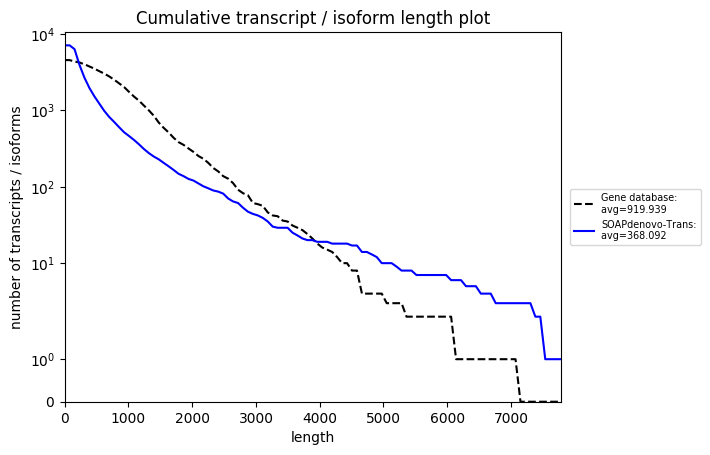
\includegraphics[width = \linewidth]{/mnt/dessertlocal/projects/transcriptome_assembly/review/evaluation/rna-quast/ath/comparison_output/transcript_length.png}
\caption{Plot showing cumulative transcript length distribution. Each point represents the number of transcripts in the assembly with the corresponding length or longer; black dashed line corresponds to the database isoforms; the plot is given in logarithmic scale.}
\end{figure}
\FloatBarrier
\clearpage


\begin{figure}[t]
\centering
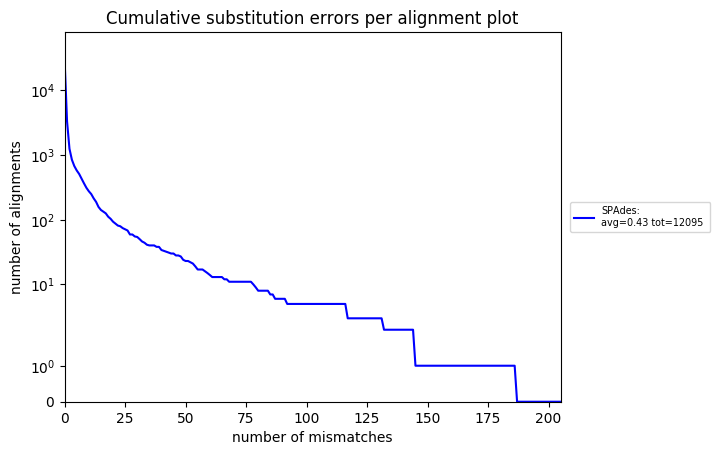
\includegraphics[width = \linewidth]{/mnt/dessertlocal/projects/transcriptome_assembly/review/evaluation/rna-quast/ath/comparison_output/mismatch_rate.png}
\caption{Plot showing cumulative substitution errors per alignment distribution. Each point represents the number of alignments with the corresponding number of mismatches or greater; the plot is given in logarithmic scale.}
\end{figure}
\FloatBarrier
\clearpage


\begin{figure}[t]
\centering
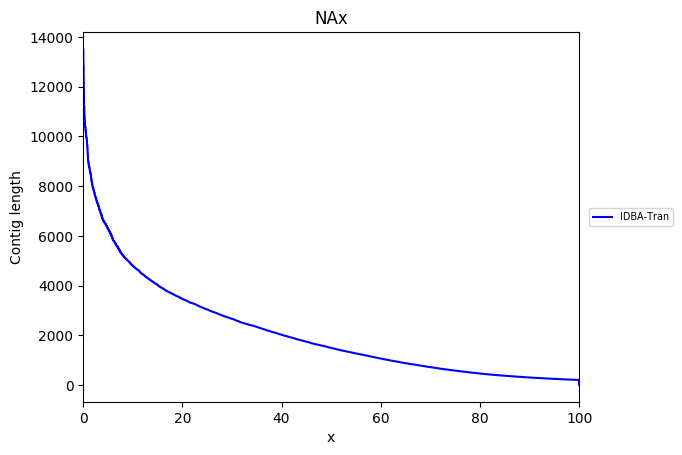
\includegraphics[width = \linewidth]{/mnt/dessertlocal/projects/transcriptome_assembly/review/evaluation/rna-quast/ath/comparison_output/NAx.png}
\caption{Nx plot for transcripts. Nx is a maximal number $N$, such that the total length of all transcripts longer than $N$ bp is at least $x\%$ of the total length of all transcripts.}
\end{figure}
\FloatBarrier
\clearpage


\begin{figure}[t]
\centering
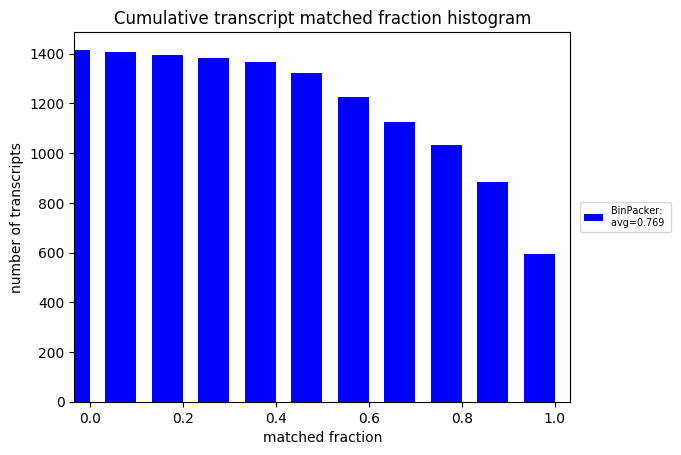
\includegraphics[width = \linewidth]{/mnt/dessertlocal/projects/transcriptome_assembly/review/evaluation/rna-quast/ath/comparison_output/x-matched.png}
\caption{Plot showing cumulative transcript match histogram. Each bar represents the number of transcripts with matched fraction equal to or greater than the value on $x$ axis; transcript matched fraction is calculated as the number of its bases covering an isoform divided by the transcript length.}
\end{figure}
\FloatBarrier
\clearpage


\begin{figure}[t]
\centering
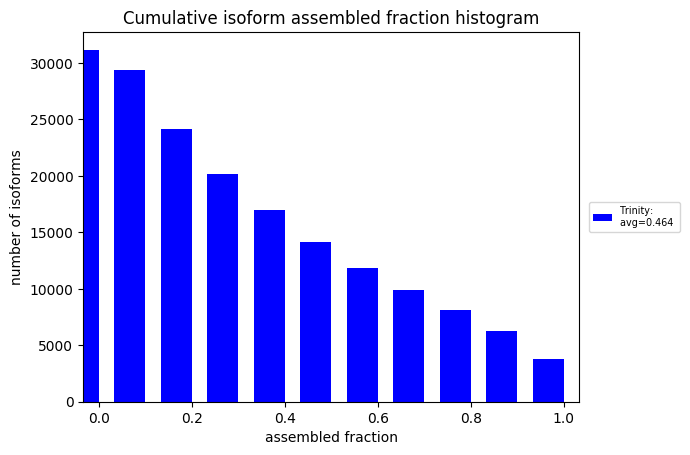
\includegraphics[width = \linewidth]{/mnt/dessertlocal/projects/transcriptome_assembly/review/evaluation/rna-quast/ath/comparison_output/x-assembled.png}
\caption{Plot showing cumulative isoform assembly histogram. Each bar represents the number of isoforms with assembled fraction equal to or greater than the value on $x$ axis; isoform assembled fraction is calculated as the maximum number of captured by single assembled transcript bases divided by the total isoform length.}
\end{figure}
\FloatBarrier
\clearpage


\begin{figure}[t]
\centering
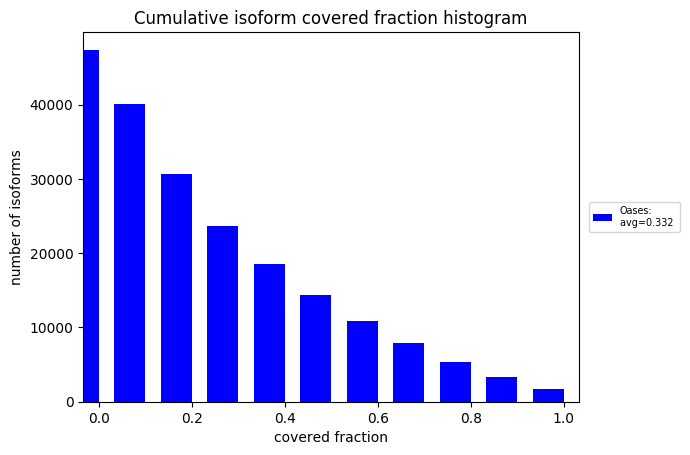
\includegraphics[width = \linewidth]{/mnt/dessertlocal/projects/transcriptome_assembly/review/evaluation/rna-quast/ath/comparison_output/x-covered.png}
\caption{Plot showing cumulative isoform coverage histogram. Each bar represents the number of isoforms with covered fraction equal to or greater than the value on $x$ axis; isoform covered fraction is calculated as the number of covered bases (by all transcripts in the assembly) divided by the total isoform length.}
\end{figure}
\FloatBarrier
\clearpage


\end{document}
